\documentclass[preprint,12pt]{elsarticle}
\usepackage{graphicx}
\usepackage{amssymb}
\usepackage{lineno}
\usepackage{booktabs}
\journal{Journal Name}

\begin{document}
\begin{frontmatter}
%% Title, authors and addresses

\title{A Mathematical model for Thelaziasis}

\author{Olmos Liceaga D., Diaz-Infante Velasco S., Acu\~na Zegarra M. A.}
\address{Universidad de Sonora}
\begin{abstract}
%% Text of abstract
In the present manuscript we present a mathematical model for thelaziasis. 
We consider outbreak studies and estimate the severity of the disease. 
We base our study on a multiple hosts ...
\end{abstract}

\begin{keyword}
Thelaziasis \sep Mathematical Model \sep Parameter Estimation \sep Basic Reproductive number
%% keywords here, in the form: keyword \sep keyword

%% MSC codes here, in the form: \MSC code \sep code
%% or \MSC[2008] code \sep code (2000 is the default)

\end{keyword}

\end{frontmatter}

%%
%% Start line numbering here if you want
%%
\linenumbers

%% main text
\section{Introduction}
\label{Section:Intro}

\noindent The disease. Hosts. What are the effects on the infected individuals. 
Where has been found. What is the vector in each case. Case studies. 
The use of a mathematical model to study a particular place.

\noindent Thelaziasis is a vector neglected disease that affects mainly mammals, including humans and in a minor scales, 
birds. The transmission takes place due to the presence of a vector which is the face fly \textit{Musca autumnalis}. 
Depending on the region this vector might vary as well as the host species.

\noindent The transmission depends upon the presence of vectors and therefore thelaziasis has a seasonal occurrence \cite{Asrat:2016}

\noindent The transmitted by the face fly \cite{Otranto:2003}. The disease has spread in animals but in humans it has been reported but in a very isolated cases \cite{Wang:2014}, \cite{Otranto:2008}, \cite{shen:2006}.\\

\noindent In \cite{Moolenbeek:1980} it was found the presence of \textit{Thelazia gulosa} and \textit{Thelazia lacrymalis} in cattle where the main responsible vector is the face fly (\textit{Musca autumnalis}) in which of larvae of \textit{Thelaszia spp} were found. Data from slaugtered cattle was collected from April to October
1978. In \cite{Lyons:2000} the authors present a survey for different diseases in equids in Kentucky USA. In their study, they found the presence \textit{Thelazia Lacrymalis} in which it is pressumed that the face fly (\textit{Musca autumnalis}) is the vector responsible for transmission. Otranto et. al. \cite{Otranto:2003} made a survey in different regions in Italy to observe the current status on dogs, cats and foxes. In their work they present the proportion of infected animals (by \textit{Thelazia Callipaeda}) in each of the regions they studied. In \cite{Dubay:2000} data about the proportions of mule deer from Wyoming and Utah by \textit{T. californiensis} was reported. Asrat \cite{Asrat:2016} sudy the prevalence of Thelaziasis in Ethiopia whereas Beitel \cite{Beitel:1974} studied the prevalence of eyeworms in the columbian black tailed deer in Oregon, USA by \textit{Thelazia californiensis}. Khedri et. al. \cite{Khedri:2016} present a one year data about infected bovine in Southeast Iran (puede ser útil).

\noindent In \cite{Ohara:1989}, the authors present a study about the prevalence and intensity of \textit{Thelazia spp} in a flies population in Alberta, Canada.


In \cite{Beitel:1974} studied the prevalence of eyeworms in the Columbian Black-Tailed Deer in Oregon. 

A special work was done in \cite{Moolenbeek:1980} were it was estimated the proportion of infected animals as well as the proportion of infected vectors.

\subsection{Some questions to explore.}
\noindent An important issue in this disease is that the propagation coincides with the presence of flies that carry the disease. If the life expectancy of the fly is reduced, then
the complete cycle of the thelazia within the vector does not complete and therefore, the 
disease no longer can be transmitted. Therefore, it might be expected that as soon as the temperature of a place of study is reduced, then the levels of the infected individuals 
with thelazia, must reach a final steady level.

\noindent In the mathematical side, analyse the model about stability, persistance, what would happen if stochasticity gets implemented? how?

\subsection{Model parameters}
\noindent Flies have a life expectancy of about 28 days, but it might live up to two months (\cite{sanchez:1998}). The first larval stage (L1) of the worm is ingested by the fly when it feeds from lachrymal secretions, where in the internal organs, the worm develops into its second (L2) and third (L3) larval stages within 21 days post infection \cite{Otranto:2003}. Other studies
\cite{Chanie:2014}, show that flies infected with \textit{Thelazia lacrymalis} can reach the infective stage in 12-15 days, while this takes 28-32 days for flies infected with \textit{T. gulosa} \cite{Chanie:2014}. Once in the infective stage, the fly releases L3 larvae into the definite host. Finally, once in the definite host, the L3 larvae matures within 3 to 6 weeks, where the new worm deposits new eggs into the definite host becoming infective \cite{Chanie:2014}. Foxes lifespan is 2 years \cite{Devenish:2014}.

\noindent We will use the model to fit two data sets. One referring to a multi-host case given by dogs and foxes and the second in a one host study, particularly the case of cattle.
%\subsubsection{Dogs and foxes}
%\noindent Foxes lifespan is about 2 years \cite{Devenish:2014}. Dogs lifespan is approximately 7 to 14 years \cite{selman:2013}.

\subsubsection{Cattle only.}
\noindent The problem can be seen as a simple host or multi-host when considering beef and milk cattle.
\noindent Some considerations about the life expectancy of the individuals. A common technique 
to detect thelazia in farming animals is done by sacrificing the animal. In this case, the infected individual is no longer part of the infection cycle and basically out of the dynamics.
In this work we consider that the sample used to observe the proportion of infected individuals is of little to neglected significance respect to the total population.

\noindent The life expectancy of beef cattle is approximately 16 to 24 months (and can be up to 30 months \cite{stanley:2003}), whereas for diary cattle is 5 to 6 years. The natural cattle life expectancy is 18 to 22 years.


\section{Mathematical Model}

\noindent Our model is based on the interaction of flies and cattle. Following the formulation in Esteva \cite{Esteva:1998} we obtain the following SI vector host model for cattle and flies.
\begin{equation}\label{Eq:SIvectorhostmodel}
\begin{array}{lcl}
\dot{S}_f&=&\Lambda_f-\frac{\beta_f}{N_c}I_cS_f-\mu_fS_f\\
\dot{L}_f&=&\frac{\beta_f}{N_c}I_cS_f-\kappa_fL_f-\mu_fL_f\\
\dot{I}_f&=&\kappa_fL_f-\mu_fI_f\\
\dot{S}_c&=&\Lambda_c-\frac{\beta_c}{N_c}I_fS_c-\mu_cS_c\\
\dot{L}_c&=&\frac{\beta_c}{N_c}I_fS_c-\kappa_cL_c-\mu_cL_c\\
\dot{I}_c&=&\kappa_cL_c-\mu_cI_c\\
\end{array}
\end{equation}
where $N_c=S_c+L_c+I_c$. For this model, the basic reproductive number is given by
 \begin{equation}
     R_0=\left(\left(\frac{k_f}{\mu_f+k_f}\right)\left(\frac{\beta_c}{\mu_f}\right)\left(\frac{k_c}{k_c+\mu_c}\right)\left(\frac{F_c\beta_f}{\mu_c} \right) \right)^{1/4}
 \end{equation}
 where $F_c=\frac{N_f^{\infty}}{N_c^{\infty}}$, $N_f^{\infty}=\frac{\Lambda_f}{\mu_f}$ and $N_c^{\infty}=\frac{\Lambda_c}{\mu_c}$. Table \ref{Table:Parameters} show the meaning and the values of the parameters considered in this study.
 
%Clearly, the root is due to the presence of the four-cycle as shown in figure (Z)
%which is the contribution of the infection cycles fox-flies and dogs-flies.\\

%About the number of cattle in a farm
%http://www.agr.gc.ca/eng/industry-markets-and-trade/canadian-agri-food-sector-intelligence/red-meat-and-livestock/red-meat-and-livestock-market-information/inventories/cattle-inventory-by-farm-type-ontario/?id=1415860000081

\begin{table*}[htb]\label{Table:Parameters}
	\begin{center}
        \begin{tabular}{cllc}
	%		\toprule
			\hline
			Parameter		&	Meaning & Interval & Reference
			\\
			\midrule
			$N_c$& Total number of &&\\
			&individuals at time $t$ &1000&This study
			\\
			$\Lambda_f$& Fly recruitment rate & & This study
			\\
			$\Lambda_c$& Cattle recruitment rate & & This study
			\\			
			$\beta_c$& Number of successful &&\\
			&contacts of a fly &&
				\\
			& that infects a cattle host &&This study
				\\
			$\beta_f$& Number of successful&&\\
			&contacts in which &&
				\\
			& a fly gets infected by a &&\\
			&cattle host &&This study
				\\
			$k_v^{-1}$	& average latency time &&\\
			&for vectors & 14-21 days &\cite{Otranto:bookchapter}
			\\
				& & 12-15 days &\\
				&&(\textit{T. Lacrymalis}) &\cite{Chanie:2014}
			\\
				& & 28-32 days&\\ 
				&&(\textit{T. Gulosa}) &\cite{Chanie:2014}
			\\
			$k_{i}^{-1}$
			&
				average latency time &&\\
				&for hosts $i=1,2$ & $\approx$ 35 days& \cite{Otranto:bookchapter}
			\\
			& & 21-42 days& \cite{Chanie:2014}
			\\			
			 $\mu_v^{-1}$	& vector average lifespan & 30-60 months&\cite{sanchez:1998}
			\\
			$\mu_c^{-1}$
			&
				cows average lifespan & 1080 days& \cite{FAOweb}
			\\
    		\bottomrule
		\end{tabular}
	\end{center}
	\caption{
		Parameter meaning and values.	}
\end{table*}


\section{Local and global stability analysis}
\noindent System \ref{Eq:SIvectorhostmodel} has two equilibrium points. The disease free equilibrium $S_1$ = $(S_{f1}^*,L_{f1}^*,I_{f1}^*,S_{c1}^*,L_{c1}^*,I_{c1}^*)$ = $(\frac{\Lambda_f}{\mu_f},0,0,\frac{\Lambda_c}{\mu_c},0,0)$ and the endemic equilibrium $S_2$ = $(S_{f2}^*,L_{f2}^*,I_{f2}^*,S_{c2}^*,L_{c2}^*,I_{c2}^*)$ = . 

\noindent Theorem. The disease free equilibrium point $S_1$ is globally asymptotically stable if $R_0<1$.
Consider the Lyapunov function
$$V(L_f,I_f,L_c,I_c)=a_1L_f+a_2I_f+a_3L_c+a_4I_c$$
$$
\begin{array}{lll}
\dot{V}(t)&=&a_1\left[\frac{\beta_f}{N_c}S_cI_c-(\mu_f+k_f)L_f\right]+a_2\left[k_fL_f-\mu_fI_f\right]\\
&&+a_3\left[ \beta_c\frac{S_cI_f}{N_c}-(k_c+\mu_c)L_c\right]+a_4\left[k_cL_c-\mu_cI_c\right]\\
&\leq& \left[\frac{a_1\beta_fN_f}{N_c}-a_4\mu_c\right]I_c+\left[a_2k_f-a_1(\mu_f+k_f)\right]L_f+\\
&&\left[a_3\beta_c-a_2\mu_f\right]I_f+\left[a_4k_c-a_3(k_c+\mu_c)\right]L_c
\end{array}
$$
Then, by taking $a_1=\frac{1}{\mu_c}\frac{k_c}{k_c+\mu_c}\frac{\beta_c}{\mu_f}\frac{k_f}{k_f+\mu_f}$, $a_2=\frac{1}{\mu_c}\frac{k_c}{k_c+\mu_c}\frac{\beta_c}{\mu_f}$, $a_3=\frac{1}{\mu_c}\frac{k_c}{k_c+\mu_c}$ and $a_4=\frac{1}{\mu_c}$, we arrive to
$$
\begin{array}{lll}
\dot{V}(t)&\leq& R_0-1,\\
\end{array}
$$
which completes the proof.

\subsection{Persistance}

\section{Discussion}

\section{Numerical Results}

    \begin{figure*}
    \centering
    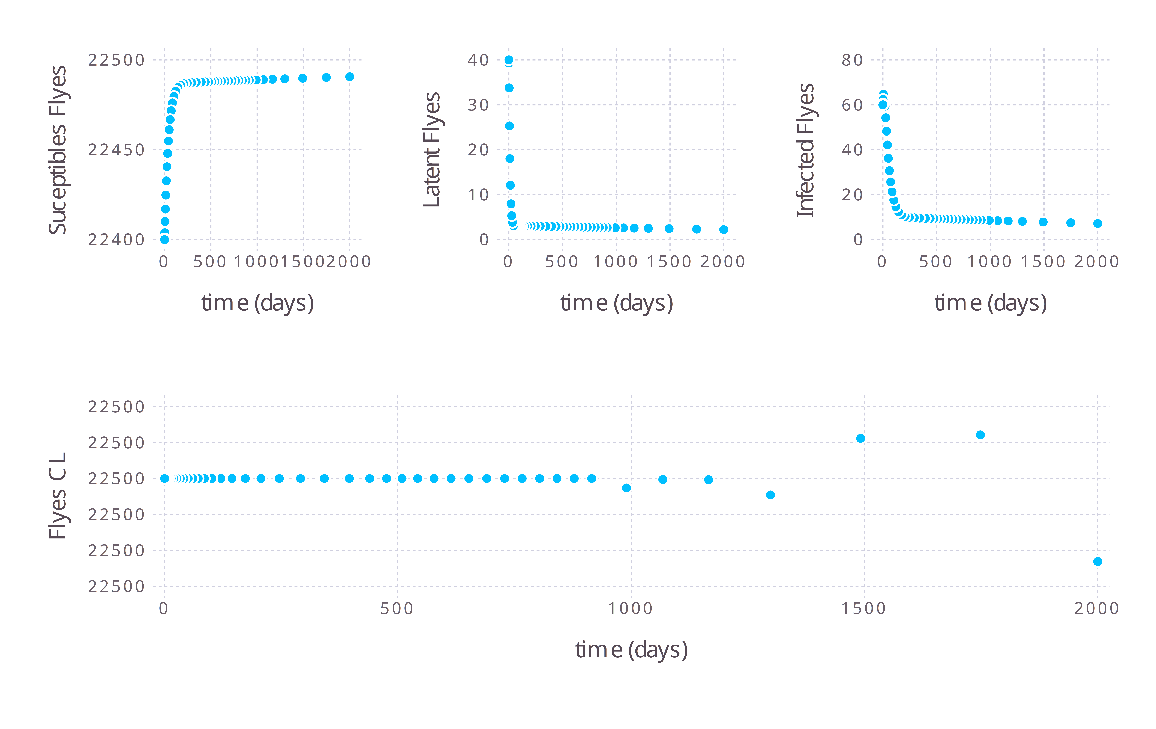
\includegraphics[width=\linewidth, keepaspectratio]{%
    Figures/flyes_disease_dynamics}
    \caption{Solution with parameters according to $R_0 < 1$.}
    \label{fig:flyesdiseasedynamics}
\end{figure*}
%
%
%
\begin{figure*}
    \centering
    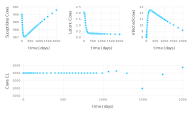
\includegraphics[width=\linewidth, keepaspectratio]{%
    Figures/cows_disease_dynamics}
    \caption{Solution with parameters according to $R_0 < 1$ 
    }
    \label{fig:cowsdiseasedynamics}
\end{figure*}


\textbf{Bibliography}
\bibliographystyle{model1-num-names}
\bibliography{thelazbiblio.bib}
\end{document}
